%************VERSUCHSANORDNUNG*************
\chapter{Experimental Setup}
\label{sec:versuchsandordnung}
The experimental work done in this thesis primarily utilized a Low-Temperature Scanning Tunneling Microscope setup (LT-STM).
This STM is composed of two distinct compartments, the preparation chamber (PC) the measurement chamber (MC).
The sample is inserted through a airlock into the preparation chamber.
In the whole system there is in a Ultra High Vacuum (UHV) at about 10$^{-11}$ - 10$^{-10}$ mbar, which is archieved by four individuall pumps.
The base Vacuum is achieved with the turbomolecular pump and the scroll pump through the airlock.
Additionally there is a titanium sublimation pump and a ion pump in the preparation room.

\monofig{width=\textwidth}{Experimental_Setup/STM_Picture_1_edited.pdf}{
    The experimental setup used, 
    A: cooling-chamber filled with Liquid Oxigen,
    B: measuring-chamber with spring suspended sample holder and tip,
    C: sputter-gun,
    D: metal-evaporater,
    E: molecule-evaporater,
    F: preparation-chamber with free movable sample holder arm,
    G: LEED system,
    H: Electronic used to monitor the function of the STM}{fig:stm_uni_kf}
%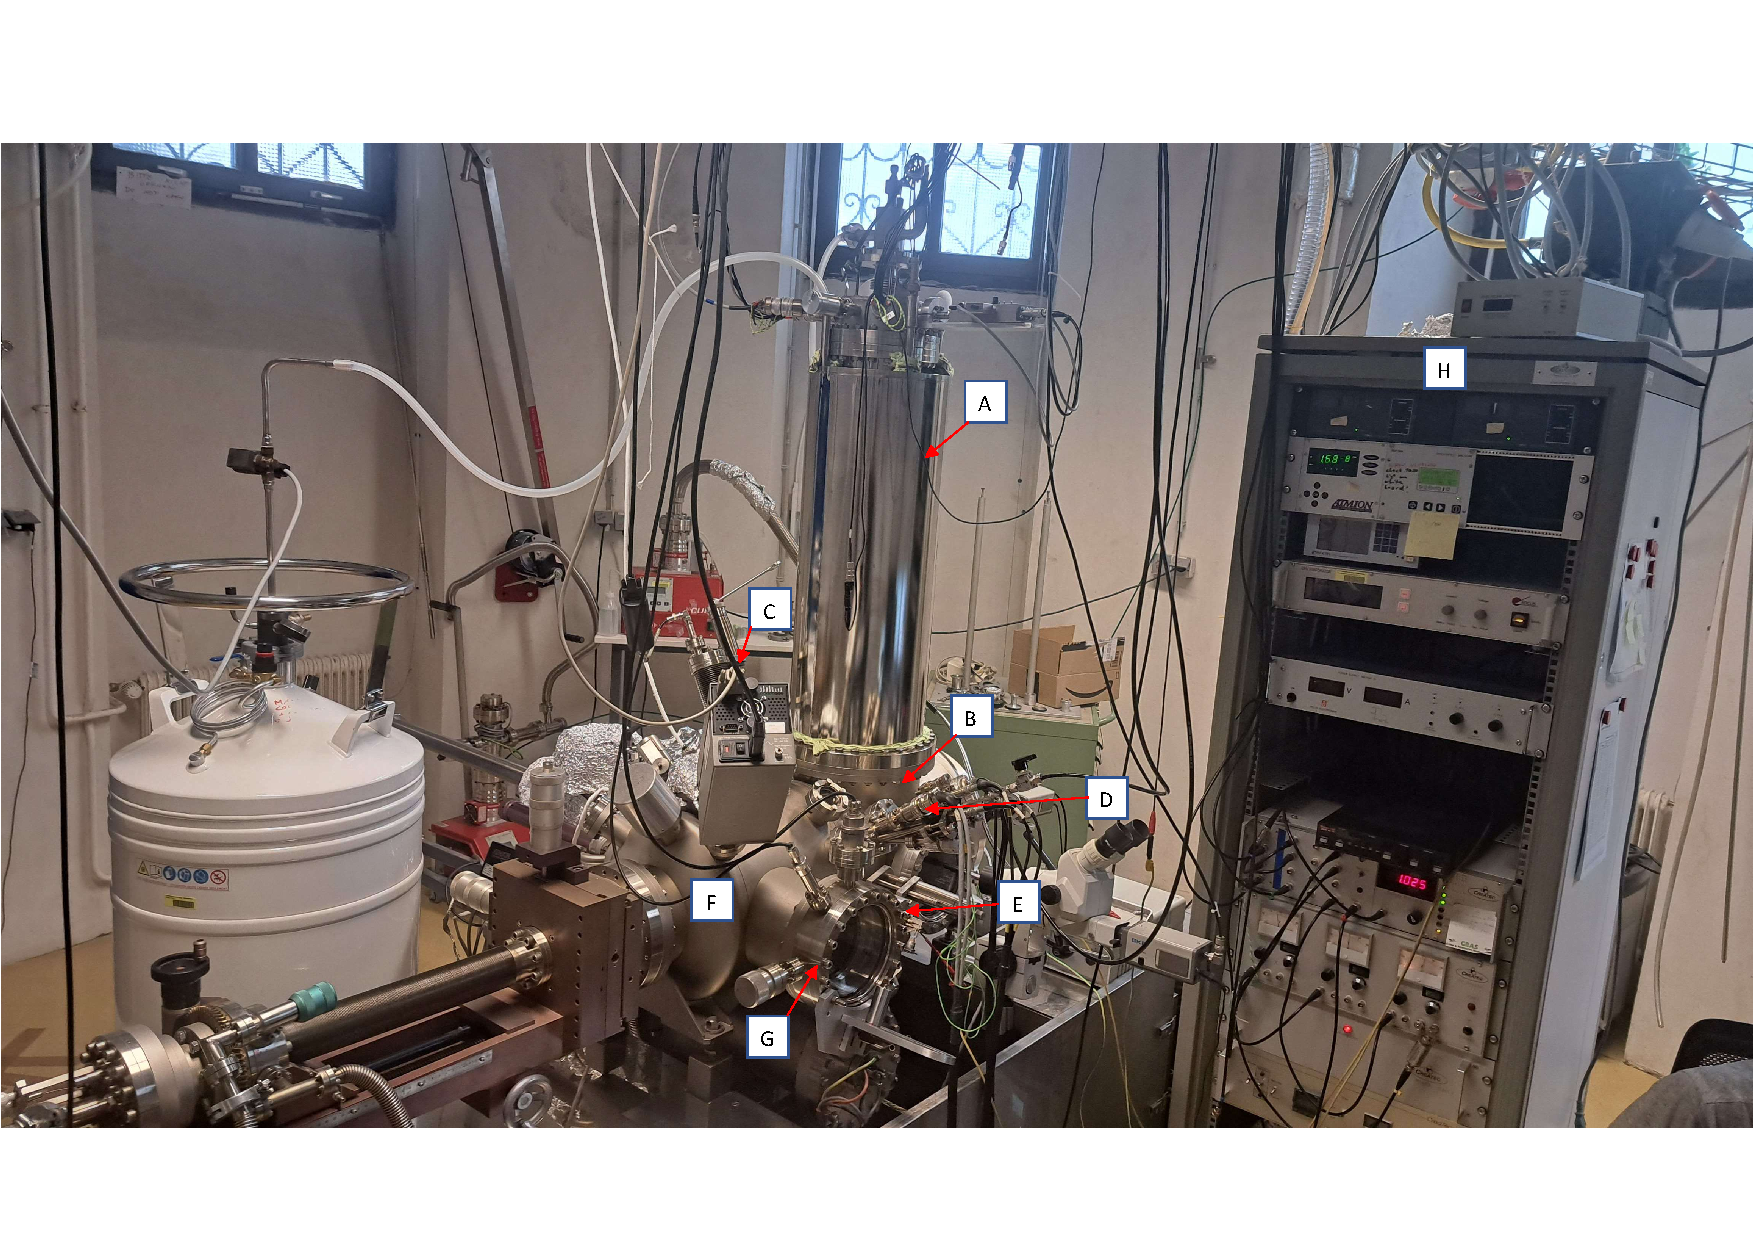
\includegraphics[width=0.9\textwidth]{Experimental_Setup/STM_Picture_1_edited.pdf}

The Probe-holder can be moved in each direction and rotated using an integrated arm in the PC.
It is also used to insert the Probe-holder into the MC.
The PC is equipped with a LEED system, which fluorescent screen can be extended. 
Additionally the PC has a metal-evaporator and organic-molecule evaporator (E-beam evaporator with a triple Knudsen cell) which are used to deposit submono- or monolayer structres onto an circular sample (10 mm x 2 mm).
This sample is mounted onto the previously mentioned Probe-holder, a Heatwaves Labs Inc. button heater with a resistive heating range of 20 K - 900 K.
The sample can also be cooled using LN2 or LHe through built-in pipe system in the manipulator arm.
A Quartz-Crystal Microbalance (QCM) with sub Angstöm precision is used to monitor the deposition thickness.
To clean the sample, an Argon sputter gun is employed, which utilizes an electric field to ionize and accelerate the argon gas.
The MC consists of a LT-STM which is surrounded by a two-shell cryostat, to which it is fixed, and two radiation shields to archieve temperatures as low as 7 K.
In this thesis the cryostat chamber was filled with LN2 which means it was operated at 75 K.
The primary measuring unit (tip and sample storage place) is vibrationally damped using a coupled spring system.


\section{Sample Preparation}
\subsection{Substrate}
The Substrate used in this thesis is a Silver (Ag) single crystal.  
Silver is a metal with 47 Protons and two stable isotopes 107Ag and 109Ag that are almost almost equally distributed.
It has an atomic radius of 1.44 \AA and it naturally crystallizes into a face centered curbic (fcc) structure with a lattice constant of a = 4.079 \AA. [\cite{PhysRev.25.753}]
The single crystal is cut along the (100) plane giving it a square surface lattice along the [011] and [01$\bar{1}$] Direction.
To insure that the surface is clean, multiple cycles of Argon-Ion Sputtering with consequent annealing were performed. 
The first preparation was done with 3x Sputtering for 5 min each and annealing at 500 C° for 3-5 min.
Later a longer sputtering time of 20 min proved more effective.  
Prior to the metal or organic adsorbtion the substate is cooled to room temperature.

\section{Magnesium Oxide (MgO)}
The crystal structure of MgO is also fcc with a lattice constant of a = 4.22 \AA [\cite{guilliatt1969lattice}], which makes it only 3.4 \% larger than Ag.
This allows the formation of somewhat larger terrases, which often break in rectangular shapes. This comes from the cubic structure of MgO.
The preparation on Ag(100) is done using a E-beam evaporator, in which a filament is heated, causing it to emit electrons.
This electrons are than accelerated using a high voltage (250-300V) onto the Magnesium probe.
The product of the emission current and acceleration voltage is the heating capacity.
To ensure a monolayer the deposition rate is measured using a Quarz-Crystal Microbalance (QCM).
A deposition rate of 1.33$\cdot$10$^2$ digit/s is established.
One digit is than deposited onto the Ag(100) substate, while Oxygen O$_2$ is being fed into the Preparation Chamber (10$^{-6}$ mbar).
After the monolayer is deposited, the sample is being slowly cooled at a cooling rate of 5 K/min.
This ensures larger terrases as MgO is known to b0reak into small islands if cooled to fast.


\section{Pentacenequinone}
Pentacenes are a organic molecule group with five linearly organised benzene rings, which share two or four neighboring carbon atoms.
The carbon atoms are sp$^2$ hybridised, which gives it a hexagonal structure in which the single- and double-bond is alternating.
At the double-bond location the $\pi$ orbital extends orthogonal to the plane in which the benzene rings are aligned.
The overlaping of neighbouring $\pi$ orbitals results in delocalized electrons across the molecule. \\
\begin{wrapfigure}{r}{0.5\textwidth}
    \centering
    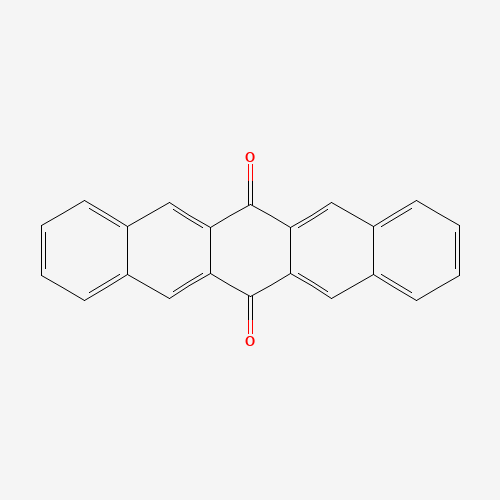
\includegraphics[width=0.49\textwidth]{graphics/6,13-Pentacenequinone.png}
    \caption{Pentacenequinone PubChem \cite{pentacenequinone}}
    \label{fig:penta}
\end{wrapfigure}
\noindent Quinone refers to the replacement of two hydrogen atoms with two oxygen atoms in a benzene ring %[\cite{NIAZ2020749}].
The two carbonyl bonds (C=O) in the observed adsorbant are located in the central ring.
Pentacene is an organic p-type semiconductor, which is used in the domain of organic electronics.
Its remarkably stable and has a high charge mobility for an organic molecule of 2.2 cm$^2$ V$^{-1}$ s$^{-1}$ [\cite{MOTA2018511}].
Pentacenequinone exibits similar properties and is used as a precursor for the synthetization of pentacene. \\
\\

\section{2-Hydrogen Phthalocyanine}
Phthalocyanines are a group of organic molecules that exibit a variety of properties.
They are characterized by a symmetric macrocyclic structure of four isoindole units [(C$_6$H$_4$)C$_2$N], which consists of a pyrole unit fused with a benzene ring. 
The isoindole units are linked by four nitrogen atoms (aza-bridges) forming a conjugated chain.
This allows a delocalization of the $\pi$ electrons along the alternating double- and single bond macrocycle.



\begin{wrapfigure}{l}{0.5\textwidth}
    \centering
    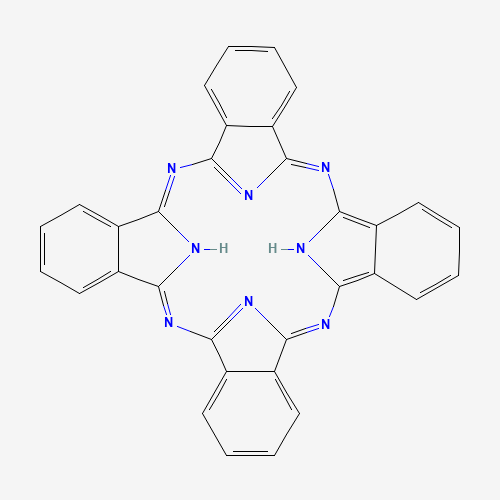
\includegraphics[width=0.49\textwidth]{graphics/Phthalocyanine.png}
    \caption{2-H Phthalocyanine PubChem \cite{phthalacyanine}}
    \label{fig:phtalo}
\end{wrapfigure}

There are more than 70 variations of the phthalocyanine, with they key difference in the substitution of different elements or transition metals (e.g. Cu$^{2+}$ and Ni$^{2+}$) in the middle of the molecule.
The physical properties can be strongly altered by the choise of different metal ions, like the adsorbtion characteristics or the geometry of the molecule itself. 
In this thesis the 2-Hydrogen Phthalocyanine is observed, which harbors, as the name already tells, two hydrogen Atoms in the middle attached to two opposing pyrole units.
Generally Phthalocyanines are remarkably chemically and thermally stable.
This can be attributed to its planar geometry and conjugation in the macrocycle.
Phthalocyanines are used as as dye for textiles and as inks because they strongly absorb light in the visable range especially in 620 - 750 nm regime, which makes them appear dark green-blue. 
Its also known for its optical, electronic and photo-electronic properties, all of which makes it a promising sensor chemiresistor.
Because of the semiconducting properties of phthalocyanins, its capability as a transistor, its use as liquid crystal display or its solar-cell applications are investigated. 